\documentclass[portrait]{a0poster}	% Document class and orientation
    \setlength{\paperwidth}{90cm}	% Poster width in cm
    \setlength{\paperheight}{120cm}	% Poster height in cm

% % Basic packages
\usepackage[utf8x]{inputenc}
\usepackage{ucs}
\usepackage[american]{babel}
\usepackage{amsmath, amsfonts, mathtools, amsthm, amssymb}
\usepackage[left=2cm,right=2cm,top=2cm,bottom=2cm]{geometry}

% Fonts and Spacing
\setlength{\parindent}{1.5em}
\setlength{\parskip}{0.5em}
\usepackage{indentfirst}
\usepackage{helvet}
\usepackage[bitstream-charter]{mathdesign}
\usepackage[T1]{fontenc}
\usepackage{textcomp}
\usepackage[frenchmath]{mathastext}

% Section Fonts
\usepackage{titlesec}
\titleformat*{\section}{\Large\bfseries\sffamily}
\titleformat*{\subsection}{\large\bfseries\sffamily}
\titleformat*{\subsubsection}{\itshape\sffamily\subsubsectionfont}

% Colors
\usepackage[dvipsnames]{xcolor}

% Headers
\usepackage{fancyhdr}
\pagestyle{fancy}
\fancyhead[RO,LE]{\rightmark}
\fancyhead[RE,LO]{}
\fancyfoot[LE,RO]{\thepage}
\fancyfoot[C]{\leftmark}

% Theorems
\makeatother
\usepackage{thmtools}
\usepackage[framemethod=TikZ]{mdframed}
\mdfsetup{skipabove=1em,skipbelow=0em}

\theoremstyle{definition}

\declaretheoremstyle[
    headfont=\bfseries\sffamily\color{ForestGreen!70!black}, bodyfont=\normalfont,
    mdframed={
        linewidth=2pt,
        rightline=false, topline=false, bottomline=false,
        linecolor=ForestGreen, backgroundcolor=ForestGreen!5,
    }
]{thmgreenbox}

\declaretheoremstyle[
    headfont=\bfseries\sffamily\color{NavyBlue!70!black}, bodyfont=\normalfont,
    mdframed={
        linewidth=2pt,
        rightline=false, topline=false, bottomline=false,
        linecolor=NavyBlue, backgroundcolor=NavyBlue!5,
    }
]{thmbluebox}

\declaretheoremstyle[
    headfont=\bfseries\sffamily\color{NavyBlue!70!black}, bodyfont=\normalfont,
    mdframed={
        linewidth=2pt,
        rightline=false, topline=false, bottomline=false,
        linecolor=NavyBlue
    }
]{thmblueline}

\declaretheoremstyle[
    headfont=\bfseries\sffamily\color{RawSienna!70!black}, bodyfont=\normalfont,
    mdframed={
        linewidth=2pt,
        rightline=false, topline=false, bottomline=false,
        linecolor=RawSienna, backgroundcolor=RawSienna!5,
    }
]{thmredbox}

\declaretheoremstyle[
    headfont=\bfseries\sffamily\color{RawSienna!70!black}, bodyfont=\normalfont,
    numbered=no,
    mdframed={
        linewidth=2pt,
        rightline=false, topline=false, bottomline=false,
        linecolor=RawSienna, backgroundcolor=RawSienna!1,
    },
    qed=\qedsymbol
]{thmproofbox}

\declaretheoremstyle[
    headfont=\bfseries\sffamily\color{NavyBlue!70!black}, bodyfont=\normalfont,
    numbered=no,
    mdframed={
        linewidth=2pt,
        rightline=false, topline=false, bottomline=false,
        linecolor=NavyBlue, backgroundcolor=NavyBlue!1,
    },
]{thmexplanationbox}

\declaretheorem[style=thmgreenbox, name=Definition]{definition}
\declaretheorem[style=thmbluebox, numbered=no, name=Example]{example}
\declaretheorem[style=thmredbox, name=Proposition]{proposition}
\declaretheorem[style=thmredbox, name=Theorem]{theorem}
\declaretheorem[style=thmredbox, name=Lemma]{lemma}
\declaretheorem[style=thmredbox, numbered=no, name=Corollary]{corollary}

\declaretheorem[style=thmproofbox, name=Proof]{replacementproof}
\renewenvironment{proof}[1][\proofname]{\vspace{-10pt}\begin{replacementproof}}{\end{replacementproof}}
\declaretheorem[style=thmexplanationbox, name=Proof]{tmpexplanation}
\newenvironment{explanation}[1][]{\vspace{-10pt}\begin{tmpexplanation}}{\end{tmpexplanation}}
\declaretheorem[style=thmblueline, numbered=no, name=Remark]{remark}

%\theoremstyle{definition}
%\newtheorem{theorem}{Theorem}[section]
%\newtheorem{corollary}[theorem]{Corollary}
%\newtheorem{lemma}[theorem]{Lemma}
%\newtheorem{remark}[theorem]{Remark}
%\newtheorem{proposition}[theorem]{Proposition}
%\newtheorem{example}{Example}[section]
%\newtheorem{definition}{Definition}[section]
%\renewcommand\qedsymbol{$\blacksquare$}

% Additional Packages
\usepackage{url}
\usepackage[colorlinks=true, allcolors=magenta, backref=page]{hyperref}
\usepackage{tikz}

% Setup
\hypersetup{
    colorlinks=false,
    pdftitle={Topology of Metric Spaces},
    pdfpagemode=FitH,
}

\usepackage[margin=1in]{geometry}	% Set poster margins in inches

\usepackage{multicol}				% Use multiple columns
    \columnsep=100pt				% Set space between columns in points
    \columnseprule=3pt 				% Set width of line between columns in points

\usepackage{graphicx}				% For adding images
\usepackage{float}					% For using float environments
\usepackage{booktabs}				% For table rules
\usepackage{palatino}				% For times font
\usepackage{lipsum}					% For generating random text

\usepackage[utf8]{inputenc}
\usepackage{ucs}
\usepackage[brazilian]{babel}
\usepackage{csquotes}
\usepackage{amsmath, amsfonts, mathtools, amsthm, amssymb}

% Fonts and Spacing
\setlength{\parindent}{1.5em}
% \setlength{\parskip}{0.5em}
\usepackage{indentfirst}
\usepackage{helvet}
\usepackage[bitstream-charter]{mathdesign}
\usepackage[T1]{fontenc}
\usepackage{textcomp}
\usepackage[frenchmath]{mathastext}
\renewcommand{\normalsize}{\Large}
\renewcommand{\large}{\Large}
\renewcommand{\Large}{\LARGE}
\renewcommand{\small}{\normalsize}
\renewcommand{\footnotesize}{\normalsize}
\renewcommand{\scriptsize}{\normalsize}
\renewcommand{\tiny}{\normalsize}
\renewcommand{\Huge}{\veryHuge}

% Section Fonts
\usepackage{titlesec}
\titleformat*{\section}{\Large\bfseries\sffamily}
\titleformat*{\subsection}{\large\bfseries\sffamily}
\titleformat*{\subsubsection}{\itshape\sffamily\subsubsectionfont}

% Colors
\usepackage[dvipsnames]{xcolor}

% Theorems
\makeatother
\usepackage{thmtools}
\usepackage[framemethod=TikZ]{mdframed}
\mdfsetup{skipabove=1em,skipbelow=0em}

\theoremstyle{definition}

\declaretheoremstyle[
    headfont=\bfseries\sffamily\color{ForestGreen!70!black}, bodyfont=\normalfont,
    mdframed={
        linewidth=2pt,
        rightline=false, topline=false, bottomline=false,
        linecolor=ForestGreen, backgroundcolor=ForestGreen!5,
    }
]{thmgreenbox}

\declaretheoremstyle[
    headfont=\bfseries\sffamily\color{NavyBlue!70!black}, bodyfont=\normalfont,
    mdframed={
        linewidth=2pt,
        rightline=false, topline=false, bottomline=false,
        linecolor=NavyBlue, backgroundcolor=NavyBlue!5,
    }
]{thmbluebox}

\declaretheoremstyle[
    headfont=\bfseries\sffamily\color{NavyBlue!70!black}, bodyfont=\normalfont,
    mdframed={
        linewidth=2pt,
        rightline=false, topline=false, bottomline=false,
        linecolor=NavyBlue
    }
]{thmblueline}

\declaretheoremstyle[
    headfont=\bfseries\sffamily\color{RawSienna!70!black}, bodyfont=\normalfont,
    mdframed={
        linewidth=2pt,
        rightline=false, topline=false, bottomline=false,
        linecolor=RawSienna, backgroundcolor=RawSienna!5,
    }
]{thmredbox}

\declaretheoremstyle[
    headfont=\bfseries\sffamily\color{RawSienna!70!black}, bodyfont=\normalfont,
    numbered=no,
    mdframed={
        linewidth=2pt,
        rightline=false, topline=false, bottomline=false,
        linecolor=RawSienna, backgroundcolor=RawSienna!1,
    },
    qed=\qedsymbol
]{thmproofbox}

\declaretheoremstyle[
    headfont=\bfseries\sffamily\color{NavyBlue!70!black}, bodyfont=\normalfont,
    numbered=no,
    mdframed={
        linewidth=2pt,
        rightline=false, topline=false, bottomline=false,
        linecolor=NavyBlue, backgroundcolor=NavyBlue!1,
    },
]{thmexplanationbox}

\declaretheorem[style=thmgreenbox, numberwithin=section, name=Definição]{definition}
\declaretheorem[style=thmbluebox, numberwithin=section, name=Exampleo]{example}
\declaretheorem[style=thmredbox, numberwithin=section, name=Teorema]{theorem}
\declaretheorem[style=thmredbox, sibling=theorem, name=Proposição]{proposition}
\declaretheorem[style=thmredbox, sibling=theorem, name=Lema]{lemma}
\declaretheorem[style=thmredbox, sibling=theorem, name=Corolário]{corollary}

\declaretheorem[style=thmproofbox, name=Proof]{replacementproof}
\renewenvironment{proof}[1][\proofname]{\vspace{-10pt}\begin{replacementproof}}{\end{replacementproof}}
\declaretheorem[style=thmexplanationbox, name=Proof]{tmpexplanation}
\newenvironment{explanation}[1][]{\vspace{-10pt}\begin{tmpexplanation}}{\end{tmpexplanation}}
\declaretheorem[style=thmblueline, numbered=no, name=Remark]{remark}

% TIKZ
\newcommand\crule[3][black]{\textcolor{#1}{\rule{#2}{#3}}}
\usepackage{pgfplots}
\pgfplotsset{width=7cm,compat=1.8}
\usepackage{pgfplotstable}
% Create a function for generating inverse normally distributed numbers using the Box–Muller transform
\pgfmathdeclarefunction{invgauss}{2}{%
  \pgfmathparse{sqrt(-2*ln(#1))*cos(deg(2*pi*#2))}%
}
\makeatletter
\pgfplotsset{
    table/.cd,
    brownian motion/.style={
        create on use/brown/.style={
            create col/expr accum={
                (\coordindex>0)*(
                    max(
                        min(
                            invgauss(rnd,rnd)*0.1+\pgfmathaccuma,
                            \pgfplots@brownian@max
                        ),
                        \pgfplots@brownian@min
                    )
                ) + (\coordindex<1)*\pgfplots@brownian@start
            }{\pgfplots@brownian@start}
        },
        y=brown, x expr={\coordindex},
        brownian motion/.cd,
        #1,
        /.cd
    },
    brownian motion/.cd,
            min/.store in=\pgfplots@brownian@min,
        min=-inf,
            max/.store in=\pgfplots@brownian@max,
            max=inf,
            start/.store in=\pgfplots@brownian@start,
        start=0
}
\makeatother

% Initialise an empty table with a certain number of rows
\pgfplotstablenew{201}\loadedtable % How many steps?
\pgfplotsset{
        no markers,
        xmin=0,
        enlarge x limits=false,
        scaled y ticks=false,
        ymin=-1, ymax=1
}
\tikzset{line join=bevel} 

\usepackage{url}
\usepackage[colorlinks=true, allcolors=magenta]{hyperref}
\usepackage{tikz}

% Title
\author{\sffamily \href{https://github.com/adairneto}{Adair Antonio da Silva Neto}}
\title{\sffamily \uppercase{Introdução às Equações Diferenciais Estocásticas}}
\date{\sffamily \today}

% \usepackage[url=false,doi=false,giveninits=true,isbn=false]{biblatex}	% Use biblatex
% 	\addbibresource{XXX_poster.bib}										% Add .bib file

% Setup
\hypersetup{
    colorlinks=false,
    pdftitle={Introdução às Equações Diferenciais Estocásticas},
    pdfpagemode=FitH,
}

\begin{document}

%%%%%%%%%%%%%%%%%%%%%%%%%%%%%%%%%%%%%%%%%%%%%%%%%%%%%%%%%%%%%%%%%%%%%%%%%%%%%%%%%%%%%%%%%%
% Title Mini-page
%%%%%%%%%%%%%%%%%%%%%%%%%%%%%%%%%%%%%%%%%%%%%%%%%%%%%%%%%%%%%%%%%%%%%%%%%%%%%%%%%%%%%%%%%%


\begin{figure}[h]
    \centering
      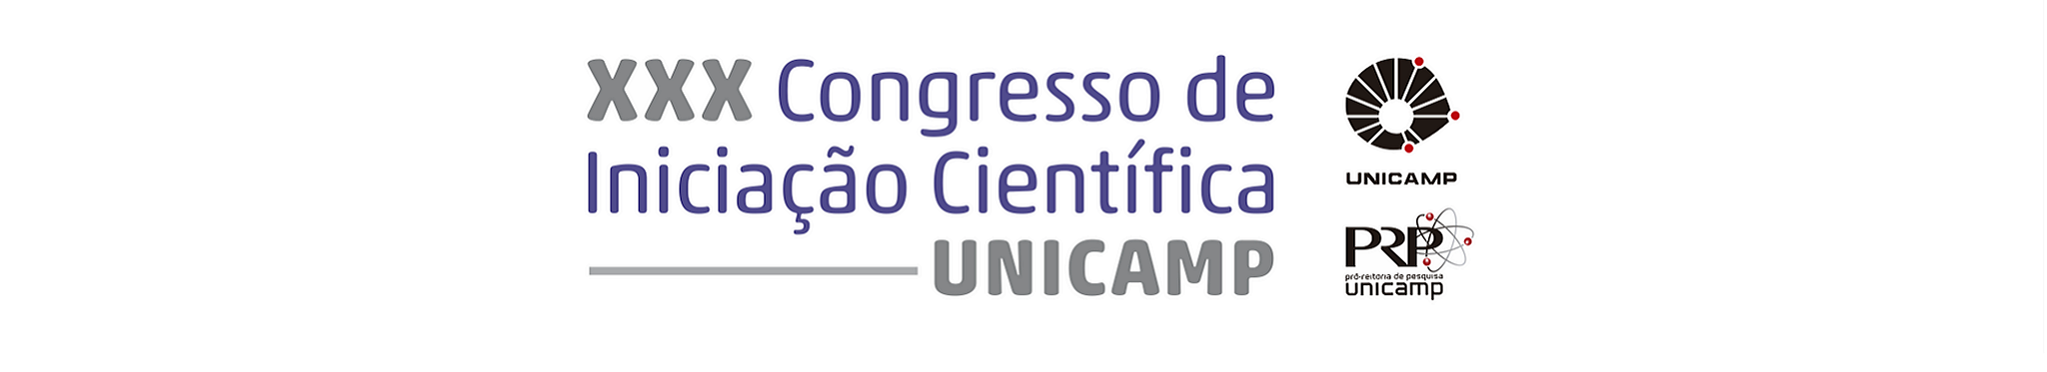
\includegraphics[width=\textwidth]{logo.png}
  \end{figure}

\begin{minipage}{\textwidth}
	% Title Area
	\begin{minipage}{\textwidth}
        \Huge\textbf{Introdução às Equações Diferenciais Estocásticas}
    
        \par\huge Adair Antonio da Silva Neto (IMECC, UNICAMP)
        \par\huge Prof. Dr. Diego Sebastián Ledesma (IMECC, UNICAMP)
        \par\huge\textbf{Palavras-chave:} Cálculo Estocástico, Movimento Browniano, Ruído Branco.
        \par\huge\textbf{Financiamento:} FAPESP
	\end{minipage}
\end{minipage}

\vspace{1cm}

%%%%%%%%%%%%%%%%%%%%%%%%%%%%%%%%%%%%%%%%%%%%%%%%%%%%%%%%%%%%%%%%%%%%%%%%%%%%%%%%%%%%%%%%%%
% Main Text 
%%%%%%%%%%%%%%%%%%%%%%%%%%%%%%%%%%%%%%%%%%%%%%%%%%%%%%%%%%%%%%%%%%%%%%%%%%%%%%%%%%%%%%%%%%

\begin{multicols}{2}

    % Summary Section
    % This section is divided into four standard subsections Background, Methods, Results and Conclusions. Either can be written as a subsection (e.g. \subsection{Background}) or just as bold-face regular text (e.g. \textbf{Background}) to have all in one paragraph. Figs or Tabs can be referenced using \ref{<figure-label>}. References can be cited using \cite{<citation-id>}
    
    \section*{Introdução}

    Uma equação que modela um processo de evolução que contém ruído, com certa aleatoriedade, seria uma equação da forma:
    \begin{equation}\label{eq:sde}
        \frac{\mathrm{d}X}{\mathrm{d}t} = b(t,X_t) + \sigma(t,X_t)\cdot \text{`ruído'}
    \end{equation}

    Problemas como esse aparecem naturalmente na biologia (modelos de crescimento populacional), física (carga em circuitos elétricos), engenharia (problemas de filtragem como o Filtro de Kalman exibido na Figura \ref{fig:kalman}) e finanças (parada ótima, portfólio ótimo e precificação de opções). 

    \begin{figure}[H]
    \centering
        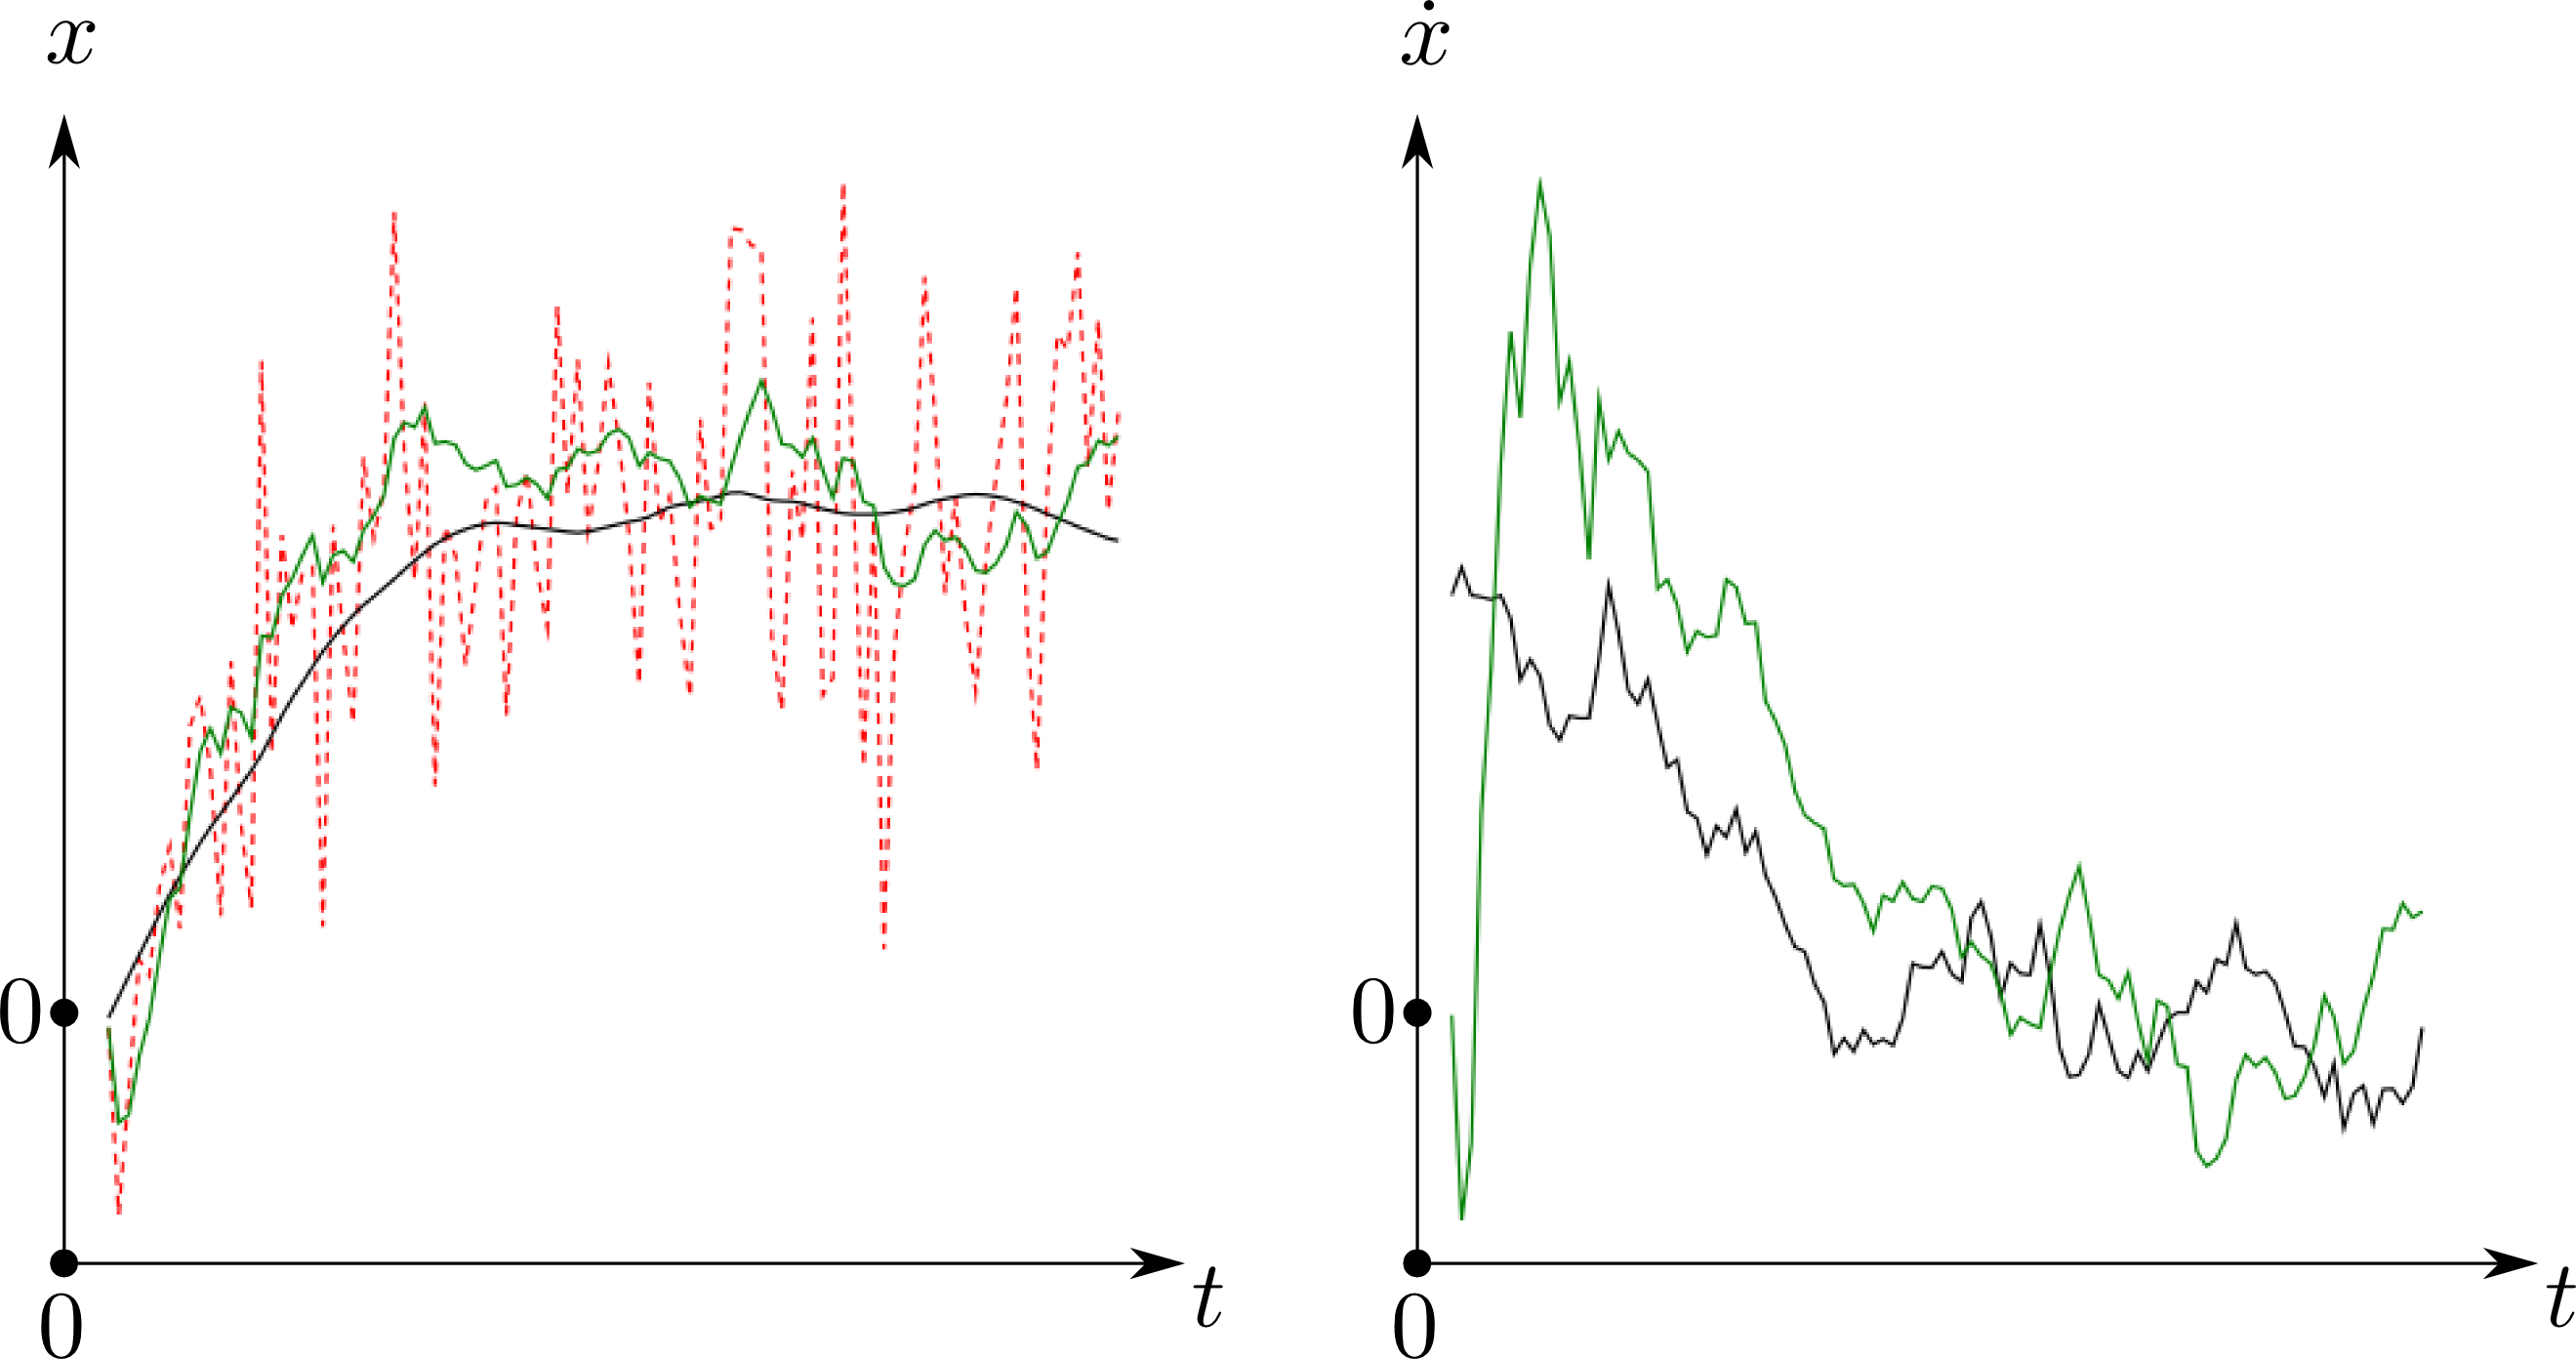
\includegraphics[width=0.4\textwidth]{Kalman.png} 
        \caption{Filtro de Kalman: $\crule[red]{0.4cm}{0.4cm}$ Dados observados; $\crule[ForestGreen]{0.4cm}{0.4cm}$ Processo filtrado; $\crule{0.4cm}{0.4cm}$ Dados reais \cite{wiki:Kalman_filter}.}
        \label{fig:kalman}
    \end{figure}

    Do ponto de vista matemático, temos que dar sentido a esse tipo de equações, pois com as ferramentas usuais do cálculo diferencial e integral não é possível tratá-las. Nosso objetivo então, neste trabalho, é dar os fundamentos que permitem começar a tratar estas equações. Em particular, definir a integral de Itô.

    \section*{Metodologia}

    Para estudar a equação \eqref{eq:sde} primeiramente damos uma forma para o `ruído' que vamos considerar. No nosso caso, vamos considerar o `ruído branco', que é um processo estocástico generalizado $W_t$ com distribuição de probabilidade gaussiana de média zero, variância finita tal que $\mathbb{E}[W_sW_t]=0$ sempre que $t\neq s$. No entanto, este processo não tem propriedades razoáveis (não tem caminhos contínuos, não é mensurável para tempo finito). Por causa disso é considerado o movimento Browniano $B_t$ que pode ser visto como um processo estocástico estacionário, com incrementos independentes e média zero tal que 
    \[
    B_t-B_s=W_s(t-s)
    \]
    para todo $t\geq s$ isto é, o `ruído branco' é a derivada em relação ao tempo do movimento Browniano. De fato, o único processo que satisfaz essas propriedades é o movimento Browniano (Figura \ref{fig:brownian_motion}). 

    \begin{figure}[h!]
    \centering
    \pgfmathsetseed{3}
    \begin{tikzpicture}[scale=1.2]
    \begin{axis}
        \addplot table [
            brownian motion = {%
                start = 0,	
                max =  0.5,
                min = -0.75
            }
        ] {\loadedtable};
        \addplot table [
            brownian motion = {%
                start =  0,
                min   = -0.5,
                max   =  0.75
            }
        ] {\loadedtable};
    \end{axis}
    \end{tikzpicture}
    \caption{Simulação de duas realizações do movimento Browniano \cite{texexchange:brownian-tikz}}
    \label{fig:brownian_motion}
    \end{figure}

    Passamos agora ao tratamento da equação. Para isso, observamos que no caso determinístico, em que não há presença de ruído, temos uma equação da forma
    \begin{equation}
        \frac{\mathrm{d} X_t}{\mathrm{d} t} = b(t, X_t), \quad X_0 = x_0
    \end{equation}

    Nesse caso, uma solução é uma função $X_t$ tal que
    \begin{equation}
        X_t - X_0 = \int_0^T b(s, X_s) \mathrm{d}s
    \end{equation}
    Essa função pode ser vista como um processo estocástico sobre um espaço de probabilidade dado por um único ponto. 

    Utilizando o formalismo acima propomos como solução à equação \eqref{eq:sde} uma identidade da forma
    \begin{equation}\label{eq:sde-sol-prop}
        X_t - X_0 = \int_0^t b(s, X_s) \mathrm{d}s + \int_0^t \sigma(s, X_s) \mathrm{d}B_s
    \end{equation}
    onde a integral da esquerda é uma integral de Lebesgue-Stieltjes, mas a integral da direita é o que vamos formalizar neste trabalho. 

    \section*{Resultados e Discussão}

    Como vimos na seção anterior queremos dar sentido à seguinte integral
    \begin{equation}\label{eq:gen_ito_integrand}
        \int_S^T f(t, \omega) \mathrm{d}B_t(\omega)
    \end{equation}
    onde $f : [0, \infty] \times \Omega \longrightarrow \textbf{R}$.

    A ideia será a seguinte: começaremos definindo a integral para as funções mais simples possíveis e depois, por aproximações e critérios de convergência, iremos defini-la para as outras classes de funções. Em particular queremos definir a integral para   a classe de funções  $\mathfrak{V}(S,T)$ que está formada por 
        \[
            f(t, \omega) : [0, \infty) \times \Omega \longrightarrow \textbf{R}
        \]
        tais que
        \begin{enumerate}
            \item A função $(t, \omega) \longrightarrow f(t, \omega)$ é $\mathfrak{B} \times \mathfrak{F}$-mensurável, onde $\mathfrak{B}$ denota a $\sigma$-álgebra de Borel em $[0, \infty)$ e $\mathfrak{F}$ é a $\sigma$-álgebra gerada pelas variáveis aleatórias $B_s$ ($s \leq t$).
            \item A função $f(t,\omega)$ é $\mathfrak{F}_t$-adaptada.
            \item $\mathbb{E} \left[ \int_S^T f(t, \omega)^2 \mathrm{d}t \right] < \infty$.
        \end{enumerate}

    Começamos então com as funções mais simples. 
    \begin{definition}[Funções elementares]
            Uma função $\varphi \in \mathfrak{V}(S,T)$ é dita \textbf{elementar} se é da forma
        \begin{equation}
            \varphi(t, \omega) = \sum_j e_j(\omega) \chi_{[t_j, t_{j+1}]}(t)
        \end{equation}
    \end{definition}

    Para as funções elementares definimos 
    \[
    \int_S^T\varphi(t, \omega)~dB_t=\sum_{j}e_j(\omega)(B_{t_{j+1}}(\omega)-B_{t_j}(\omega)).
    \]
    As funções elementares são importantes porque são densas em $\mathfrak{V}(S,T)$ como garante o seguinte resultado.
    \begin{theorem}
    Se $g\in \mathfrak{V}(S,T)$  então existe uma sequência de funções elementares $\varphi_n\in \mathfrak{V}(S,T)$ tal que $\varphi_n\to g$ em $L^2(P)$
    \end{theorem}

    E, a partir disso, podemos definir a integral \eqref{eq:gen_ito_integrand} com a seguinte definição.

    \begin{definition}[Integral de Itô]
        Seja $f \in \mathfrak{V}(S,T)$, então a \textbf{Integral de Itô} de $f$, de $S$ a $T$ é
        \begin{equation}
            \int_S^T f(t, \omega) \mathrm{d}B_t(\omega) = \lim_{n \to \infty} \int_S^T \varphi_n (t, \omega)  \mathrm{d}B_t(\omega)
        \end{equation}
        onde o limite é em $L^2(P)$ e $( \varphi_n )$ é uma sequência de funções elementares tais que
        \[
            \mathbb{E} \left[ \int_S^T (f(t, \omega) - \varphi_n(t, \omega))^2 \mathrm{d}t \right] \longrightarrow 0
        \] 
        quando $n \to \infty$.
    \end{definition}

    Com a integral de Itô já bem definida, enunciaremos a Isometria de Itô e um corolário, listaremos algumas propriedades e, por fim, daremos um exemplo do cálculo dessa integral.

    \begin{theorem}[Isometria de Itô]
        Para toda função $f \in \mathfrak{V}(S,T)$,	
        \begin{equation}
            \mathbb{E}\left[\left( \int_S^T f(t,\omega) \mathrm{d}B_t(\omega) \right)^2 \right] = \mathbb{E} \left[\int_S^T f(t,\omega)^2 \mathrm{d}t \right]
        \end{equation}
    \end{theorem}

    \begin{corollary}\label{cr:ito}
        Se $f(t, \omega) \in \mathfrak{V}(S,T)$, $f_n(t, \omega) \in \mathfrak{V}(S,T)$ e
        \[
            \mathbb{E}\left[\left( \int_S^T f_n(t,\omega) - f(t, \omega) \right)^2 \mathrm{d}t \right] \longrightarrow 0
            \]
        quando $n \to \infty$, então
        \begin{equation}
            \int_S^T f_n(t, \omega) \mathrm{d}B_t(\omega) \longrightarrow \int_S^T f(t, \omega) \mathrm{d} B)t(\omega)
        \end{equation}
        em $L^2(P)$ conforme $n \to \infty$.
    \end{corollary}

    De fato, a integral de Itô possui as propriedades esperadas de uma integral e, além disso, tem média zero e é $\mathfrak{F}_T$-mensurável.

    \begin{theorem}[Propriedades]
        Seja $f, g \in \mathfrak{V}(0,T)$ e $0 \leq S < U < T$. Então
        \begin{enumerate}
            \item $\int_S^T f \mathrm{d}B_t = \int_S^U f \mathrm{d}B_t + \int_U^T f \mathrm{d}B_t$ para $\omega$ em quase toda parte.
            \item $\int_S^T (cf + g) \mathrm{d}B_t = c \int_S^T f \mathrm{d}B_t + \int_S^T g \mathrm{d}B_t$ onde $c \in \textbf{R}$.
            \item $\mathbb{E} \left[ \int_S^T f \mathrm{d}B_t \right] = 0$.
            \item $\int_S^T f \mathrm{d}B_t$ é $\mathfrak{F}_T$-mensurável.
        \end{enumerate}
    \end{theorem}

    \begin{example}
        Queremos calcular a integral
        \[
            \int_0^T B(t) \mathrm{d}B(t)
        \]
            
        \textbf{Passo 1.} Seja
        \[
            \varphi_n(t) = \sum_{i=0}^{n-1} B_n(t_i^n)[B_n(t_{i+1}^n) - B_n(t_i^n)]
        \]
        uma sequência de funções elementares. Então,
        \begin{equation*}
            \begin{aligned}
                \mathbb{E} \left[ \int_0^T (\varphi_n - B_s)^2 \mathrm{d}s \right]
                &= \mathbb{E} \left[ \sum_j \int_{t_j}^{t_{j+1}} (B_j - B_s)^2 \mathrm{d}s \right]
                = \sum_j \int_{t_j}^{t_{j+1}} (s - t_j)^2 \mathrm{d}s \\
                &= \sum_j \frac{1}{2} \left(t_{j+1} - t_j \right)^2 \longrightarrow 0 \, \text{ quando } \Delta t_j \to 0
            \end{aligned}
        \end{equation*}
        
        Isto é, pela continuidade de $B(t)$, $\varphi_n(t)$ converge para $B(t)$ quase certamente quando $\Delta t_j \to 0$.
        
        \textbf{Passo 2.} Agora note que
        \begin{equation*}
            \begin{aligned}
                B_n(t_i)[B_n(t_{i+1}) - B_n(t_i)] &= B_n(t_{i+1}) B_n(t_i) - B_n^2(t_i) + B_n^2(t_{i+1}) - B_n^2(t_{i+1}) \\
                &= \frac{1}{2} [B_n^2(t_{i+1}) - B_n^2(t_i) - (B_n(t_{i+1}) - B_n(t_i))^2 ]
            \end{aligned}
        \end{equation*}
        
        \textbf{Passo 3.} Com esses dois resultados e o corolário \eqref{cr:ito}, podemos reescrever a integral original como
        \[
            \int_0^T \varphi_n(t) \mathrm{d}B(t) = \frac{1}{2} \sum_{i=0}^{n-1} \left[ B_n^2(t_{i+1}) - B_n^2(t_i) \right] - \frac{1}{2} \sum_{i=0}^{n-1} \left[ B_n(t_{i+1}) - B_n(t_i) \right]^2
        \]
        
        \textbf{Passo 4.} Como a primeira soma é uma soma telescópica e a segunda soma converge em probabilidade para $T$ pela variação quadrática do movimento Browniano, temos que
        \[
            \int_0^T \varphi_n(t) \mathrm{d}B(t) = \frac{1}{2} B^2(t) - \frac{1}{2} B^2(0) - \frac{1}{2}T = \frac{1}{2} B^2(t) - \frac{1}{2}T 
        \]
        
        Logo, a integral converge em $L^2(P)$ para
        \begin{equation}
            \int_0^T B(t) \mathrm{d}B(t) = \lim_{n \to \infty} \int_0^T \varphi_n(t) \mathrm{d}B(t) = \frac{1}{2} B^2(t) - \frac{1}{2}T 
        \end{equation}
    \end{example}

    % O próximo resultado afirma que a integral de Itô é um martingale e apresenta uma importante desigualdade.

    % Mas antes disso, o que é um martingale? 

    % \begin{definition}[Martingale]
    % 	Um processo estocástico $\{M_t \}$ on $(\Omega, \mathfrak{F}, P)$ é chamado de \textbf{martingale} com respeito à filtração $\mathfrak{M}_t$ se 
    % 	\begin{enumerate}
    % 		\item $M_t$ é $\mathfrak{M}_t$-mensurável para todo $t$.
    % 		\item $\mathbb{E}[|M_t|] < \infty$ para todo $t$.
    % 		\item $\mathbb{E}[M_s | \mathfrak{M}_t] = M_t$ para todo $s \geq t$.
    % 	\end{enumerate}
    % \end{definition}

    % Intuitivamente, um martingale é um processo estocástico no qual o valor esperado de qualquer ponto no futuro é igual ao valor esperado do processo no momento presente.

    \section*{Conclusões}

    Apresentamos um formalismo para a modelagem de processos de evolução com ruído a partir do movimento Browniano. Vimos que o conceito de solução clássico não funciona para esse formalismo e foi proposta uma nova interpretação. Como resultado disso, foi necessário construir uma nova teoria de integração e, com isso, a integral de Itô. Estudamos as propriedades dessa nova integral. 

    A partir disso será possível avançar em questões mais elaboradas, como por exemplo: A equação \eqref{eq:sde} tem solução? Sob quais hipóteses? Como podemos estudar o comportamento da solução?
    
    % Reference section
    \nocite{*}
    \bibliographystyle{alpha}
    \bibliography{XXX_poster.bib}
    
\end{multicols}

\end{document}